\documentclass[11pt,a4paper]{article}

\usepackage[T1]{fontenc}
\usepackage{amsmath}
\usepackage{amssymb}
\usepackage{graphicx}
\usepackage[margin=2.4cm]{geometry}
\usepackage{booktabs}
\usepackage{array}
\usepackage{tabularx}
\usepackage{hyperref}

\hypersetup{colorlinks=true,linkcolor=black,citecolor=black,urlcolor=blue}

% ---------------------------------------------------------------- shorthands
\newcommand{\px}{\partial_x}
\newcommand{\py}{\partial_y}
\newcommand{\dd}[2]{\frac{\partial #1}{\partial #2}}
\newcommand{\ddd}[2]{\frac{\partial^2 #1}{\partial #2^2}}
\newcommand{\lap}{\nabla^2}
\newcommand{\grad}{\nabla}
\newcommand{\bvec}[1]{\mathbf{#1}}
\newcommand{\code}[1]{\texttt{#1}}
\newcolumntype{L}{>{\raggedright\arraybackslash}X}

\emergencystretch=3em
\setlength{\parskip}{0.45em}
\setlength{\parindent}{0pt}
\renewcommand{\topfraction}{0.9}
\renewcommand{\bottomfraction}{0.7}
\renewcommand{\textfraction}{0.07}
\renewcommand{\floatpagefraction}{0.75}
\setcounter{topnumber}{3}
\setcounter{totalnumber}{4}

\title{Piecewise potential-vorticity inversion on the sphere\\[2mm]
\large Method, step by step}
\author{\code{pv\_inversion\_spherical}}
\date{}

\begin{document}
\maketitle

\begin{abstract}
\noindent
This document states the equations the package solves, the steps by which it
solves them, and how the calculation differs from the limited-area Fortran chain
that solves the same system. Every number quoted comes from the example runs
that ship with the package.
\end{abstract}

\tableofcontents

% =============================================================================
\section{What is solved}
\label{sec:what}

\textbf{Vertical coordinate.} The Exner function,
\begin{equation}
\Pi = C_p\left(\frac{p}{p_0}\right)^{\kappa},
\qquad
\kappa = \frac{R_d}{C_p} = \frac{2}{7},
\label{eq:exner}
\end{equation}
with $C_p=1004.5$~J~kg$^{-1}$~K$^{-1}$, $R_d=287.0$~J~kg$^{-1}$~K$^{-1}$,
$p_0=1000$~hPa. $\Pi$ decreases upward and equals $C_p$ at 1000~hPa. In this
coordinate hydrostatic balance is linear in the potential temperature, and its
$\Pi$-derivative is the static stability:
\begin{equation}
\dd{\Phi}{\Pi} = -\theta ,
\qquad
S = -\dd{\theta}{\Pi} = \ddd{\Phi}{\Pi} .
\label{eq:hydrostatic}
\end{equation}

\textbf{Horizontal operators.} With $\lambda,\varphi$ longitude and latitude
and $a=6.371\times10^{6}$~m,
$\px=(a\cos\varphi)^{-1}\partial_\lambda$, $\py=a^{-1}\partial_\varphi$, and
for a vector $(F_x,F_y)$ and a scalar $s$
\begin{equation}
\begin{gathered}
\grad\cdot\bvec{F} = \px F_x + \py F_y - \frac{\tan\varphi}{a}F_y ,
\qquad
\bvec{k}\cdot\grad\times\bvec{F} = \px F_y - \py F_x + \frac{\tan\varphi}{a}F_x ,\\
\lap s = \px\px s + \py\py s - \frac{\tan\varphi}{a}\py s .
\end{gathered}
\label{eq:ops}
\end{equation}
The wind is the rotational wind of a streamfunction,
$\bvec{V}=\bvec{k}\times\grad\psi$, so $u=-\py\psi$, $v=\px\psi$ and
$\zeta=\lap\psi$. The Coriolis parameter that enters the operator is the
floored, equator-symmetric $f^{*}$ of Step~1.

\textbf{Potential vorticity.} Ertel's $q=\rho^{-1}\boldsymbol{\eta}\cdot\grad\theta$,
made hydrostatic and written on Exner surfaces, is (2.2) of Davis and Emanuel
(1991),
\begin{equation}
q = -\frac{g\kappa\Pi}{p}
\left(
\eta\,\dd{\theta}{\Pi}
- \frac{1}{a\cos\varphi}\dd{v}{\Pi}\dd{\theta}{\lambda}
+ \frac{1}{a}\dd{u}{\Pi}\dd{\theta}{\varphi}
\right),
\label{eq:pvhydro}
\end{equation}
$\eta=f+\zeta$ the vertical absolute vorticity. Replacing the shear of the
total wind by that of the rotational wind and eliminating $\theta$ with
\eqref{eq:hydrostatic} gives their (2.3). Divided through by the leading
factor, the field the inversion works with is
\begin{equation}
\hat q \;=\; q\,\frac{p}{g\kappa\Pi}
\;=\; \left(f^{*}+\lap\psi\right)\ddd{\Phi}{\Pi}
 \;-\; \grad\!\left(\dd{\psi}{\Pi}\right)\cdot\grad\!\left(\dd{\Phi}{\Pi}\right),
\qquad
\frac{p}{g\kappa\Pi} = \left(\frac{p}{p_0}\right)^{1-\kappa}\frac{p_0}{\kappa\,g\,C_p}.
\label{eq:pvsolved}
\end{equation}
This factor is the whole of the unit conversion; everything else in the solver
is SI. Values are quoted in PVU, $1~\text{PVU}=10^{-6}$~m$^2$~K~kg$^{-1}$~s$^{-1}$.

\textbf{Balance.} Charney (1955, p.~24) writes the divergence equation, with
the divergent wind omitted, as
\begin{equation}
\lap\psi + \grad\psi\cdot\grad f
 - \frac{2}{f}\left[
   \left(\frac{\partial^2\psi}{\partial x\,\partial y}\right)^{\!2}
   - \ddd{\psi}{x}\ddd{\psi}{y}
 \right]
 = \frac{\lap\phi}{f} ,
\label{eq:charney}
\end{equation}
which multiplied through by $f$ is (1.3) of Davis (1992), and in spherical
coordinates (2.1) of Davis and Emanuel (1991). It is close to gradient-wind
balance and is solvable for $\psi$ where $\lap\phi/f + f/2>0$. The package
solves it in the exact spherical form obtained by taking the divergence of the
momentum equation on the sphere,
\begin{equation}
\lap\Phi = N(\psi),
\qquad
N(\psi) = \grad\cdot\left[\left(f^{*}+\zeta\right)\grad\psi\right]
 - \tfrac12\lap\left|\grad\psi\right|^2 ,
\label{eq:Nform}
\end{equation}
in which every term is a divergence or a Laplacian of a product formed on the
grid. On the sphere this differs from the plane form by the curvature term,
\begin{equation}
\grad\cdot\left(\zeta\grad\psi\right) - \tfrac12\lap\left|\grad\psi\right|^2
 = 2\det\left(\mathrm{Hess}\,\psi\right) - \frac{\left|\grad\psi\right|^2}{a^2}.
\label{eq:curvature}
\end{equation}
The quadratic part of $N$ comes from the symmetric bilinear form
\begin{equation}
B(a,b) = \grad\cdot\left(\zeta_a\grad b\right)
 + \grad\cdot\left(\zeta_b\grad a\right)
 - \lap\left(\grad a\cdot\grad b\right)
 = \zeta_a\zeta_b - \left(D_{1a}D_{1b} + D_{2a}D_{2b}\right)
 - \frac{2\,\grad a\cdot\grad b}{a^2},
\label{eq:polarised}
\end{equation}
$D_1,D_2$ the two deformation components, so that the tangent of the balance
row at a reference $\tilde\psi$ is $\grad\cdot(f^{*}\grad\psi')+B(\tilde\psi,\psi')$
and its principal symbol has eigenvalues $f^{*}+\tilde\zeta\mp\tilde D$,
$\tilde D=(\tilde D_1^2+\tilde D_2^2)^{1/2}$. The row is elliptic where the
absolute vorticity exceeds the deformation, $(f^{*}+\tilde\zeta)^2>\tilde D^2$,
which is Charney's condition in another form. $\tilde D$ is read off
\eqref{eq:polarised} with $a=b$, from spectral operations alone.

\textbf{The coupled system.} On each interior level the two relations hold
together, for the two fields $(\Phi,\psi)$:
\begin{align}
\lap\Phi &= \grad\cdot\left[\left(f^{*}+\lap\psi\right)\grad\psi\right]
 - \tfrac12\lap\left|\grad\psi\right|^2 ,
\label{eq:sys1}\\[1mm]
\hat q &= \left(f^{*}+\lap\psi\right)\ddd{\Phi}{\Pi}
 - \grad\!\left(\dd{\psi}{\Pi}\right)\cdot\grad\!\left(\dd{\Phi}{\Pi}\right) .
\label{eq:sys2}
\end{align}
The balance row \eqref{eq:sys1} couples $\Phi$ and $\psi$ on each level; the
potential-vorticity row \eqref{eq:sys2} couples the levels vertically through
$\Phi_{\Pi\Pi}$ and the shear terms. Davis and Emanuel (1991, p.~1934) state
that (2.1) and (2.3) form a complete system for $\Phi$ and $\Psi$ given $q$.
Both rows are quadratic: \eqref{eq:sys1} in $\psi$, \eqref{eq:sys2} bilinear in
$(\psi,\Phi)$. The system is elliptic where $f^{*}+\zeta>0$, $S>0$ and the
balance row's condition above holds.

\textbf{Boundary conditions.} At the top and the bottom,
\begin{equation}
\dd{\Phi}{\Pi} = -\theta_B \ \ \text{(lower half level)},
\qquad
\dd{\Phi}{\Pi} = -\theta_T \ \ \text{(upper half level)},
\qquad
\dd{\psi}{\Pi} = -\frac{\theta-\langle\theta\rangle}{f^{*}} \ \ \text{(both)},
\label{eq:bc}
\end{equation}
$\langle\cdot\rangle$ the area mean. The streamfunction condition is the
thermal-wind form of the hydrostatic one, $\Phi\simeq f\psi$, with the
horizontally uniform part of $\theta$ removed because it carries no flow, and
the division by $f^{*}$ made before any horizontal gradient is taken. There is
no lateral boundary: the domain is the whole sphere, and the only additional
conditions are the gauges of Step~3.

\textbf{The levels.} Nine pressure levels. The two outermost carry boundary
potential temperature on the half levels next to them (near 925 and 140~hPa);
the seven between carry potential vorticity and are the unknowns.
\begin{center}
\small
\begin{tabular}{rrlrr}
\toprule
$p$ [hPa] & $\Pi$ [J~kg$^{-1}$~K$^{-1}$] & carries &
$\delta_k$ [J~kg$^{-1}$~K$^{-1}$] & $p/(g\kappa\Pi)$ \\
\midrule
1000 & 1004.5000 & boundary $\theta_B$ & ---     & ---    \\
 850 &  958.9234 & interior $\hat q$   & $-48.66$ & 31.63 \\
 700 &  907.1774 & interior $\hat q$   & $-67.45$ & 27.53 \\
 500 &  824.0269 & interior $\hat q$   & $-67.02$ & 21.65 \\
 400 &  773.1305 & interior $\hat q$   & $-55.95$ & 18.46 \\
 300 &  712.1246 & interior $\hat q$   & $-48.58$ & 15.03 \\
 250 &  675.9784 & interior $\hat q$   & $-38.95$ & 13.19 \\
 200 &  634.2263 & interior $\hat q$   & $-77.85$ & 11.25 \\
 100 &  520.2782 & boundary $\theta_T$ & ---     & ---    \\
\bottomrule
\end{tabular}
\end{center}
$\delta_k=\tfrac12(\Pi_{k+1}-\Pi_{k-1})$ is the half-span of the vertical
stencil at level $k$, negative because $\Pi$ descends. A ten-level set adds
150~hPa. The unknown vector of the coupled system is therefore
$(\Phi_k,\psi_k)$ on the seven interior levels, and the sources are the seven
$\hat q_k$ and the two boundary temperatures.

% =============================================================================
\section{The steps}
\label{sec:steps}

\subsection{Step 1: input and the sphere}
\label{sec:step1}

\textbf{Input.} Two states on the same northern-hemisphere grid and the same
nine levels, an \emph{event} and the \emph{climatology} it is measured
against: geopotential height $z$, temperature $T$, and the wind $u,v$, each
$(9,n_{\text{lat}},n_{\text{lon}})$, bottom-up, latitude ascending from the
equator, longitude ascending from zero. The walkthrough event is the ERA5
blocking ridge of 8~January~2025, centre 43.5~N 226.5~E, on a $61\times240$
grid (Figure~\ref{fig:event}); its 500~hPa height anomaly at the centre is
272~m. Where a level lies below ground, $T$, $u$ and $v$ are carried down
unchanged and the height is continued hydrostatically,
$z_k = z_{k+1} + (R_d\bar T/g)\ln(p_{k+1}/p_k)$.

\textbf{The mirror.} The operator is global, so the hemisphere is extended to
the sphere as an \emph{even} function of latitude, in two passes. The wind is
first mirrored as the vector it is, $u$ even and $v$ odd, and its vorticity is
taken; that vorticity is then mirrored as an even scalar, and $\psi$ and the
rotational wind used downstream are built from it. Height and temperature are
mirrored evenly from the outset. With every coefficient and source even, the
operator commutes with the reflection $\varphi\to-\varphi$, the solution is
exactly even, and its northern half solves the northern problem under a
condition of no meridional gradient at the equator.

\textbf{The Coriolis parameter.} $|f|$ has a corner at the equator that would
appear inside $\grad f$ in the balance term; it is smoothed,
\begin{equation}
f^{*} = 2\Omega\sqrt{\sin^2\varphi + \sin^2\varphi_0},
\qquad \varphi_0 = 12^\circ ,
\label{eq:fstar}
\end{equation}
so that $f^{*}=3.0322\times10^{-5}$~s$^{-1}$ at the equator, the value of
$|f|$ at 12~N.

\textbf{The equatorial weight.} The mirrored mean state is continuous but not
smooth at the equator. The quadratic terms of the operator are multiplied by
the weight
\begin{equation}
w = x^3\left(10 - 15x + 6x^2\right),
\qquad
x = \mathrm{clip}\!\left(\frac{|\varphi|-5^\circ}{20^\circ-5^\circ},\,0,\,1\right),
\label{eq:weight}
\end{equation}
which is zero equatorward of 5~N, one poleward of 20~N, and twice
differentiable at both ends. It multiplies the \emph{products} the quadratic
terms are built from (Step~3), never a source or a solution.
\begin{center}
\small
\begin{tabular}{lrrrrrrrrr}
\toprule
latitude [deg N] & 0.5 & 1 & 2 & 5 & 10 & 10.5 & 15 & 20 & 30 \\
\midrule
$f^{*}/|f|$ & 23.85 & 11.95 & 6.04 & 2.59 & 1.56 & 1.52 & 1.28 & 1.17 & 1.08 \\
weight $w$ & 0 & 0 & 0 & 0 & 0.21 & 0.26 & 0.79 & 1.00 & 1.00 \\
\bottomrule
\end{tabular}
\end{center}

\textbf{The solver grid.} Every product, coefficient and derivative is formed
on a Gauss--Legendre grid with no pole row and an even number of latitudes, so
no row lies on the equator. For a triangular truncation $L$ the grid has
$\lfloor(3L+1)/2\rfloor+1$ latitudes, rounded up to even, and the next power of
two of at least twice that in longitude: the three-halves rule, which
represents products of two fields truncated at $L$ without aliasing. Read the
other way, a grid of $n_{\text{lat}}$ rows carries $L=2n_{\text{lat}}/3-1$:
$96\times192$ gives T63 (the walkthrough), $128\times256$ gives T84 (the
catalogue). Scalars move from the data grid to the solver grid through the
spectrum; winds are carried as $u\cos\varphi$ and $v\cos\varphi$, which are
band limited where the components are not.

\begin{figure}[htbp]
\centering

\includegraphics[width=0.85\linewidth]{figures/fig01_event.png}
\caption{Step 1, the event: 250\,hPa wind speed and the 500\,hPa height anomaly
against the climatology, drawn on a 40-degree disc about the centre. The
difference between the two states is what is decomposed.}
\label{fig:event}
\end{figure}

\begin{figure}[htbp]
\centering

\includegraphics[width=\linewidth]{figures/fig04_mirror.png}
\caption{Step 1, the sphere. Left: the 250\,hPa streamfunction on the global
grid, the southern half the mirror of the northern. Centre: the Coriolis floor
as the ratio $f^{*}/|f|$. Right: the weight $w$ on the operator's quadratic
products across the equatorial band.}
\label{fig:mirror}
\end{figure}

\subsection{Step 2: Pass A/B, the observed state}
\label{sec:step2}

\textbf{Streamfunction.} The vorticity is formed from the wind by quadrature
against the derivatives of the Legendre functions, so the $\tan\varphi$ term of
\eqref{eq:ops} is carried without being evaluated, and the streamfunction is
the exact inverse Laplacian, coefficient by coefficient:
\begin{equation}
\psi_{nm} = \frac{\zeta_{nm}}{-n(n+1)/a^2}, \qquad n\ge1 ,
\label{eq:invlap}
\end{equation}
with the global constant $n=0$, which carries no wind, set to zero. No
relaxation and no boundary value enter. On the walkthrough event the
rotational wind at 250~hPa has 31.0~m~s$^{-1}$ rms over the hemisphere against
29.8 for the full wind (Figure~\ref{fig:psi}).

\textbf{Potential vorticity.} The source \eqref{eq:pvsolved} is evaluated from
the observed $(\psi,\Phi)$ with the operator's own stencils
(\code{pv\_source="operator"}, the default), so that the observed pair
satisfies the discrete potential-vorticity row exactly:
\begin{itemize}
\itemsep0.1em
\item $\Phi_{\Pi\Pi}$ by the three-point non-uniform second difference of the
      geopotential on all nine levels,
      \begin{equation}
      \ddd{F}{\Pi}\bigg|_k = b^{\text{lo}}_k F_{k-1} + b^{\text{c}}_k F_k + b^{\text{hi}}_k F_{k+1},
      \quad
      b^{\text{c}}_k = \frac{-2}{\delta^{+}_k\delta^{-}_k},\;
      b^{\text{hi}}_k = \frac{2}{\delta^{+}_k\delta^{2}_k},\;
      b^{\text{lo}}_k = \frac{2}{\delta^{-}_k\delta^{2}_k},
      \label{eq:stencil}
      \end{equation}
      $\delta^{+}_k=\Pi_{k+1}-\Pi_k$, $\delta^{-}_k=\Pi_k-\Pi_{k-1}$,
      $\delta^{2}_k=\Pi_{k+1}-\Pi_{k-1}$; exact for quadratics in $\Pi$, with
      rows summing to zero;
\item the boundary temperatures as the hydrostatic differences of that
      geopotential across the half levels,
      \begin{equation}
      \theta_B = -\frac{\Phi_{850}-\Phi_{1000}}{\Pi_{850}-\Pi_{1000}},
      \qquad
      \theta_T = -\frac{\Phi_{100}-\Phi_{200}}{\Pi_{100}-\Pi_{200}} ;
      \label{eq:thetahalf}
      \end{equation}
\item the shear terms $\partial\psi/\partial\Pi$ and $\partial\Phi/\partial\Pi$
      by centred first differences over the interior levels which, at the first
      and last interior level, reach the operator's ghosts of Step~3 rather than
      the observed 1000 and 100~hPa fields.
\end{itemize}
The limited-area convention, plain centred differences of $\theta$ and of the
wind over the full level set with the boundary temperature as the mean of the
two levels beside the half level, is kept as \code{pv\_source="data"}; on the
walkthrough event the two differ by 5--14\% of the potential vorticity level
by level and by 1.4~K rms at the bottom boundary and 2.6~K at the top. The
250~hPa anomaly of the event ranges from $-5.59$ to $8.02$~PVU
(Figure~\ref{fig:pv}).

\textbf{Input checks.} A run stops if the geopotential decreases with height
at more than 1\% of points, if $\theta$ decreases with height at more than
5\%, or if the geopotential and the temperature are not hydrostatically
consistent: the area mean of the boundary temperature the geopotential implies
\eqref{eq:thetahalf}, over the mean of the two adjacent levels' $\theta$, must
lie in 0.7--1.4 at the top. For the walkthrough event and its climatology
alike the ratio is 1.002 at the bottom and 0.995 at the top.

\begin{figure}[htbp]
\centering

\includegraphics[width=0.85\linewidth]{figures/fig02_streamfunction.png}
\caption{Step 2, the streamfunction recovered from the observed wind at
250\,hPa (left) and its Laplacian, the relative vorticity (right).}
\label{fig:psi}
\end{figure}

\begin{figure}[htbp]
\centering

\includegraphics[width=0.85\linewidth]{figures/fig03_pv.png}
\caption{Step 2, Ertel potential vorticity of the event: the 250\,hPa map and
a vertical section through the centre longitude, the tropopause visible as the
crowding of the contours.}
\label{fig:pv}
\end{figure}

\subsection{Step 3: Pass C, the total balanced state}
\label{sec:step3}

The coupled system \eqref{eq:sys1}--\eqref{eq:sys2}, with the observed
$\hat q$ (floored at 0.01~PVU, the amount added given back to the unclamped
points by area weight), $\theta_B$ and $\theta_T$ as data, is solved for the
balanced $(\Phi_{\text{bal}},\psi_{\text{bal}})$ on the seven interior levels
by Newton's method. Because both rows are quadratic, the Jacobian is the
linearised operator that the pieces of Step~4 use, evaluated at the current
iterate.

\textbf{The linearised operator.} At a reference state
$(\tilde\psi,\tilde\Phi)$, with $\tilde\zeta=\lap\tilde\psi$,
\begin{align}
M_1[\Phi',\psi'] &= \lap\Phi' - \grad\cdot\left(f^{*}\grad\psi'\right) - T[\psi'],
\qquad
T[\psi'] = w\,\tilde\zeta\,\zeta' + w\,s\left[B(\tilde\psi,\psi') - \tilde\zeta\,\zeta'\right],
\label{eq:M1}\\[1mm]
M_2[\Phi',\psi'] &= A\,\ddd{\Phi'}{\Pi} + S\,\lap\psi'
 - \grad\!\left(\dd{\tilde\psi}{\Pi}\right)\cdot\grad\!\left(\dd{\Phi'}{\Pi}\right)
 - \grad\!\left(\dd{\tilde\Phi}{\Pi}\right)\cdot\grad\!\left(\dd{\psi'}{\Pi}\right)
 + (1-w)\,\tilde\zeta\,\big\langle\Phi'_{\Pi\Pi}\big\rangle ,
\label{eq:M2}
\end{align}
with $A=f^{*}+w\tilde\zeta$ the absolute vorticity, $S=\langle\tilde S\rangle +
w(\tilde S-\langle\tilde S\rangle)$ the static stability $\tilde S=\tilde\Phi_{\Pi\Pi}$
tapered to its level mean, the reference shear gradients multiplied by $w$, and
$s$ the deformation limiter below. Poleward of 20~N, $w=1$; with $s=1$ the
rows are (2.10)--(2.11) of Davis and Emanuel (1991) in divergence form:
$\lap\Phi'=\grad\cdot[(f^{*}+\tilde\zeta)\grad\psi']+\grad\cdot[(\lap\psi')\grad\tilde\psi]
-\lap(\grad\tilde\psi\cdot\grad\psi')$. The vertical second difference is
\eqref{eq:stencil} with the ghosts folded in: substituting
\begin{equation}
\Phi_0 = \Phi_1 + \theta_B(\Pi_1-\Pi_0),
\qquad
\Phi_{N-1} = \Phi_{N-2} - \theta_T(\Pi_{N-1}-\Pi_{N-2})
\label{eq:ghosts}
\end{equation}
into the end rows folds one coupling weight onto the diagonal and moves the
boundary temperature to the right-hand side as $\theta_B/\delta_1$ at the first
interior level and $-\theta_T/\delta_{N-2}$ at the last. The centred first
differences inside the cross terms reach the same ghosts, the streamfunction's
being \eqref{eq:bc}.

\textbf{The residual.} The Newton residual is evaluated through the operator
itself,
\begin{equation}
F(x) = M_{x/2}[x] - b_{x/2},
\label{eq:Fmid}
\end{equation}
the operator frozen at half the state applied to the whole state, less the
right-hand side assembled at the same half state. For a quadratic system this
is the exact residual (the midpoint identity of Step~4), and the Jacobian
$M_x$ is then the derivative of exactly the system the residual measures,
floors, weight and limiter included.

\textbf{Gauge.} A constant added to $\psi$ on any level carries no wind, and a
single global constant added to $\Phi$ passes through the vertical stencil, so
the operator has a null space of dimension $n_{\text{int}}+1$. The balance row
is a sum of divergences, so its $n=0$ coefficient vanishes identically; that
slot is overwritten with the level mean of $\psi'$, pinned to zero. A rank-one
term on the potential-vorticity row, proportional to the column mean of the
$n=0$ coefficient of $\Phi'$ with a scale built from $f^{*}$ and the vertical
stencil alone, removes the global constant. The observed state's level-mean
geopotential is removed before the first step.

\textbf{Scaling.} The unknown column is $(\Phi,\;f_0\psi)$ with
$f_0=10^{-4}$~s$^{-1}$ and the rows are $(r_1,\;(f_0/\bar S_k)\,r_2)$, $\bar S_k$
the level-mean static stability, so that a single Krylov tolerance means the
same thing on both rows. This is a similarity transform.

\textbf{Preconditioner.} Freezing $A$ and $S$ at their level means $A_k,S_k$
and dropping the cross and deformation terms leaves a system that spherical
harmonics diagonalise horizontally, $\lambda_n=-n(n+1)/a^2$, and eliminating
$\psi$ exactly gives one tridiagonal problem per harmonic,
\begin{equation}
\left[\mathrm{diag}\!\left(\frac{A^2}{S}\right)T + \lambda_n I\right]\Phi
 = \frac{A}{S}\,r_2 + r_1 ,
\qquad
\psi = \frac{1}{A}\left(\Phi - \frac{r_1}{\lambda_n}\right),
\label{eq:precond}
\end{equation}
$T$ the folded vertical second difference. The reduced matrix is negative
definite for every $n\ge1$; the inverses are precomputed once per event. The
$n=0$ block uses the rank-one-corrected operator for $\Phi$ and reads the
streamfunction mean off the balance row.

\textbf{Linear solve.} One preconditioned GMRES per Newton step, restart 60,
relative tolerance $10^{-8}$, a budget of 800 operator applications; a solve
counts as converged only if an independently recomputed $\|b-Mx\|/\|b\|$ is
below $10^{-7}$.

\textbf{Floors.} $A\ge10^{-6}$~s$^{-1}$ and $S\ge10^{-4}$ (SI), applied by
the \code{parity} rule: a value below a tenth of the floor is set to the
floor. The clamped area fraction per level is reported.

\textbf{Deformation limiter.} Where the reference deformation exceeds the
absolute vorticity the linearised balance row is not elliptic. The safety net
scales the deformation part of \eqref{eq:M1} alone,
\begin{equation}
s = \min\!\left(1,\ \frac{(1-m)\,A}{w\,\tilde D}\right),
\qquad m = 0.05 ,
\label{eq:limiter}
\end{equation}
so the symbol becomes $A\mp s\,w\,\tilde D\ge mA$ while the vorticity part
$\tilde\zeta\zeta'$, on which gradient-wind balance rests, is untouched. The
limiter is a frozen field, one factor per interior level on the grid. By
default (\code{adaptive}) it starts as one everywhere and is brought in only on
evidence of a fold: an inner solve that runs out of its budget, a line search
that fails, or stagnation (three or more halvings with a residual not halved).
Each refresh takes the pointwise minimum of the limiter in force, the observed
state's and the current iterate's; at most six refreshes are allowed and each
is counted. It was needed by 2 of the 50 catalogue events, on at most 17\% of
a level's area. The pieces take the limiter the total inversion converged with.

\textbf{Line search and stopping.} Backtracking by halves, at most eight
times, accepting the first step with
$\|F(x+\sigma\delta)\|\le(1-10^{-4}\sigma)\|F(x)\|$; if none passes, the best
step tried is applied. After every step the two boundary levels are rebuilt
from \eqref{eq:ghosts} and \eqref{eq:bc}. The iteration stops when the largest
geopotential increment over the interior grid is below $0.981$~m$^2$~s$^{-2}$
($g\times0.1$~m) and that step's line search succeeded, with a cap of 20
steps. Beside the increment, the report carries the residuals of the equations
\emph{as posed} (no weight, floors or limiter) at the returned state: the
balance row inverted to a height in metres and the potential-vorticity row in
PVU, globally and poleward of 20~N, together with the area fraction per level
on which the linearised balance row is not elliptic there.

\textbf{Numbers.} The walkthrough event converges in five steps with
increments of 308, 21.6, 1.50, 0.12 and 0.037~m (Figure~\ref{fig:convergence}),
no backtracking, no inner solve short of tolerance and the limiter never
brought in; the posed potential-vorticity equation is met to 0.0040~PVU rms
poleward of 20~N, the posed balance equation to $1$--$4\times10^{-7}$~s$^{-1}$
of equivalent vorticity there, and the linearised balance row is not elliptic
at the returned state on 1.5\% of the area at 850~hPa rising to 14.1\% at
300~hPa. Across the fifty catalogue events at T84, 45 converge in four steps,
three in five, and the two that meet a fold bring the limiter in once and
finish in nine and ten; the potential-vorticity residual poleward of 20~N is
0.0043~PVU rms at the median, 0.0019 to 0.0079 across events.

\begin{figure}[htbp]
\centering

\includegraphics[width=0.9\linewidth]{figures/fig05_convergence.png}
\caption{Step 3, the nonlinear iteration on the walkthrough event: the Newton
increment in metres of height against the 0.1\,m tolerance (left), and the
Krylov iterations of the nine piece solves of Step~4 against the one frozen
operator (right).}
\label{fig:convergence}
\end{figure}

\subsection{Step 4: Pass D, the pieces}
\label{sec:step4}

\textbf{The frozen operator.} The perturbation is measured from the observed
climatological mean, $\psi'=\psi_{\text{bal}}-\bar\psi$,
$\Phi'=\Phi_{\text{bal}}-\bar\Phi$, and the operator
\eqref{eq:M1}--\eqref{eq:M2} is frozen once at the midpoint,
\begin{equation}
\tilde\psi = \bar\psi + \tfrac12\psi' ,
\qquad
\tilde\Phi = \bar\Phi + \tfrac12\Phi' ,
\qquad
A = f^{*}+w\tilde\zeta,
\qquad
\tilde S = \ddd{\tilde\Phi}{\Pi},
\label{eq:midpoint}
\end{equation}
its two boundary levels rebuilt as the ghosts \eqref{eq:ghosts}, \eqref{eq:bc}
of the midpoint temperature $\bar\theta+\tfrac12\theta'$. For a quadratic
nonlinearity $N$ and a bilinear $B$ the midpoint linearisation is an identity,
\begin{align}
N(\bar x + x') - N(\bar x) &= DN\!\left(\bar x + \tfrac12 x'\right)\!\left[x'\right],
\label{eq:idquad}\\
B(\bar x + x',\,\bar y + y') - B(\bar x,\bar y)
 &= B\!\left(x',\,\bar y + \tfrac12 y'\right)
  + B\!\left(\bar x + \tfrac12 x',\,y'\right),
\label{eq:idbilin}
\end{align}
so $M_{\tilde x}$ applied to the full perturbation returns exactly the
difference between the nonlinear system at the total state and at the mean.
Because $w$ and $s$ multiply symmetric products, the identities hold with the
weight and the limiter on. This is the full-linear method of Davis (1992):
the pieces of this operator sum to the all-sources solve by construction.

\textbf{The sources.} Nine, one per piece: the potential-vorticity anomaly on
each of the seven interior levels, with $\theta_n=0$ on both boundaries, and
the temperature anomaly on each boundary, with $\hat q_n=0$ in the interior.
The interior anomaly is the difference of the event and mean fields floored
\emph{separately} at $10^{-5}$~PVU; the boundary anomalies are plain
differences. The right-hand side of a piece is linear in its source:
\begin{equation}
b_1 = 0,
\qquad
b_2 = \hat q_n
 - A\,\Theta_n
 - (1-w)\,\tilde\zeta\,\big\langle\Theta_n\big\rangle
 + \grad\!\left(\dd{\tilde\psi}{\Pi}\right)\cdot\grad\Phi^{\text{gh}}_{n}
 + \grad\!\left(\dd{\tilde\Phi}{\Pi}\right)\cdot\grad\psi^{\text{gh}}_{n},
\label{eq:rhs}
\end{equation}
$\Theta_n$ the folded boundary source ($\theta_{B,n}/\delta_1$,
$-\theta_{T,n}/\delta_{N-2}$) and $\Phi^{\text{gh}}_n$, $\psi^{\text{gh}}_n$
the ghost parts of the first differences inside the cross terms, the
streamfunction's built by \eqref{eq:bc} from the piece's own boundary anomaly.
The boundary temperature therefore enters twice, through the stability term
and through the shear terms, from one vertical operator.

\textbf{One linear solve per piece.} Each piece is one preconditioned GMRES
solve against the same operator and the same preconditioner, with the Krylov
settings of Step~3; on the walkthrough event the nine pieces take 44 to 61
iterations (Figure~\ref{fig:convergence}, right). The solved interior is
extended to the two boundary levels hydrostatically: $\Phi_n$ by
\eqref{eq:ghosts} and $\psi_n$ by the thermal-wind ghost \eqref{eq:bc}, both
from the piece's own boundary anomaly, zero for an interior piece.

\textbf{Induced wind.} From each piece's streamfunction, spectrally:
$u_n=-\py\psi_n$, $v_n=\px\psi_n$, with $u\cos\varphi$ and $v\cos\varphi$
synthesised from a table of Legendre combinations that divides by nothing.
For the walkthrough event the rms of the 250~hPa wind induced by each piece over
the hemisphere is
\begin{center}
\small
\begin{tabular}{lccccccccc}
\toprule
piece & 1000 $\theta$ & 850 & 700 & 500 & 400 & 300 & 250 & 200 & 100 $\theta$ \\
\midrule
rms [m~s$^{-1}$] & 3.83 & 2.07 & 1.80 & 1.91 & 3.19 & 7.21 & 10.29 & 11.73 & 14.66 \\
\bottomrule
\end{tabular}
\end{center}
against an observed anomaly of 21.09~m~s$^{-1}$ (Figure~\ref{fig:perlevel}).
The top-boundary piece is the largest single piece: a planetary-scale
temperature anomaly at the lid has a deep, nearly barotropic response, part of
which cancels against the interior upper-level pieces.

\begin{figure}[htbp]
\centering

\includegraphics[width=0.74\linewidth]{figures/fig06_per_level.png}
\caption{Step 4, the wind at 250\,hPa induced by each source. Shading is the
source that drives the piece, potential vorticity on the seven interior levels
and potential temperature on the two boundaries; arrows are the rotational
wind it induces at 250\,hPa, with the arrow scale set panel by panel.}
\label{fig:perlevel}
\end{figure}

\subsection{Step 5: grouping and the scale split}
\label{sec:step5}

\textbf{Groups.} Pieces are linear in their sources, so groups are sums of
pieces, exactly, formed after the solve:
\begin{center}
\small
\begin{tabular}{ll}
\toprule
group & sources \\
\midrule
surface & 1000~hPa boundary potential temperature \\
lower & potential vorticity at 850, 700, 500~hPa \\
upper & potential vorticity at 400, 300, 250, 200~hPa and the 100~hPa boundary \\
\bottomrule
\end{tabular}
\end{center}
On the walkthrough event they come to 3.83, 3.68 and 20.68~m~s$^{-1}$ rms at
250~hPa (Figure~\ref{fig:groups}).

\textbf{Planetary and eddy.} With \code{--pieces scale} the upper source is
split further by horizontal scale into \code{upper\_p} and \code{upper\_e},
and the split is applied to the \emph{source}, additively, so that the parts
still sum to the piece they came from:
\begin{enumerate}
\itemsep0.1em
\item the upper-level anomaly (400--200~hPa) is filtered on the whole circle to
      zonal orders 1--4, a selection of spherical-harmonic orders;
\item the object is seeded at the most negative filtered point within
      $\pm10^\circ$ latitude and $\pm20^\circ$ longitude of the tracked centre,
      and the contour is 0.35 of the local minimum there;
\item the object is the three-dimensional six-connected component of the
      filtered field below that contour holding the seed, sought inside the
      event's $\pm30^\circ\times\pm60^\circ$ box, whose columns run around the
      circle;
\item the masked field is filtered again to orders 1--4; that is the planetary
      part, and the eddy part is the remainder of the upper anomaly;
\item the top boundary temperature is split the same way, with the mask of the
      highest interior level.
\end{enumerate}
The four pieces \code{surface}, \code{lower}, \code{upper\_p}, \code{upper\_e}
then exhaust the sources; the contour, the local minimum and the object's area
fraction are written to the output metadata.

\begin{figure}[htbp]
\centering

\includegraphics[width=\linewidth]{figures/fig07_groups.png}
\caption{Step 5, the pieces grouped into surface, lower and upper
contributions to the 250\,hPa rotational wind, beside the observed anomalous
rotational wind. Colour and arrow scales are set panel by panel; the rms in
each title is what to compare.}
\label{fig:groups}
\end{figure}

\subsection{Step 6: closure and residual}
\label{sec:step6}

\textbf{Closure.} The sum of the nine pieces is compared with the solve that
has all nine sources present at once; the two agree to rounding, because
every piece is $M^{-1}b_n$ against one operator and $\sum_n M^{-1}b_n =
M^{-1}\sum_n b_n$. On the walkthrough event the relative difference is
$1.7\times10^{-8}$, on the 79~N event of Step~7 $5.1\times10^{-9}$. This is
checked on every run.

\textbf{Residual.} The sum of the pieces against the \emph{observed} anomalous
rotational wind leaves the part the balance equations do not represent: the
anomaly of the unbalanced and divergent flow. It is not a wall response, there
being no wall, and it is stored under its own name. On the walkthrough event
the pieces sum to 20.01~m~s$^{-1}$ rms at 250~hPa over the hemisphere against
an observed anomaly of 21.09, leaving 3.10~m~s$^{-1}$, 15\% of the anomaly
(Figure~\ref{fig:closure}); at 79~N the figures are 19.10 against 20.25,
leaving 4.17, or 21\%. Over the fifty catalogue events, on the common patch at
400--200~hPa, the residual is 0.26~m~s$^{-1}$ of a 10.12~m~s$^{-1}$ anomaly,
2.6\%.

\textbf{What the pieces close against.} Three quantities are kept apart. The
pieces sum to the all-sources linear solve exactly. They differ from the
balanced perturbation $\psi_{\text{bal}}-\bar\psi$ by the response to the
mean state's own imbalance, because the mean enters as observed rather than
balanced: 4.14~m~s$^{-1}$ rms at 250~hPa on the walkthrough event. And the
balanced total state differs from the observed rotational wind by the event's
own departure from balance: 4.97~m~s$^{-1}$ out of 30.99. The residual above
is the difference of the last two.

\begin{figure}[htbp]
\centering

\includegraphics[width=\linewidth]{figures/fig08_closure.png}
\caption{Step 6, the observed anomalous rotational wind at 250\,hPa (left),
the sum of the nine pieces (centre), and what is left over, the unbalanced and
divergent part (right).}
\label{fig:closure}
\end{figure}

\subsection{Step 7: output on any patch}
\label{sec:step7}

Nothing in Steps~1--6 refers to where the event is: the operators are global,
the grid has no pole row and no metric factor is divided by. The Greenland
event at 79~N that ships with the package is inverted by the same calculation
in five Newton steps to a final increment of 0.003~m
(Figure~\ref{fig:polar}). Two croppings are written.

\textbf{The geographic patch.} An event-centred box of half-widths
$30^\circ\times60^\circ$ on the data's own regular grid, longitudes wrapped.
Rows past the pole are NaN, because a column of the box carries one longitude
and the far side of the pole belongs to another. The pole row itself is NaN
($|\cos\varphi|\le10^{-8}$): the wind is defined there but its eastward and
northward components are not. Rows south of the data's first row, the mirror
scaffold, are NaN as well. The two-dimensional fields are the column average
over 400--200~hPa weighted by $\exp(-z/H)$, $H=7000$~m, divided by the weight
of the valid levels only.

\textbf{The rotated patch} (\code{--rotated-track}). The frame is rotated so
that the centre sits on its equator; the wind is carried as its Cartesian
components, which are smooth across the pole, sampled by cubic interpolation
on the rotated grid and rotated into the local frame. The patch is complete
for any centre, the pole included, and has the same shape for every event.
Figure~\ref{fig:polarcap} shows both croppings of two events at 55 and 80~N.

\textbf{The key contract.} One compressed \code{npz} per event, keys named
so that a loader enumerating pieces by the prefix \code{u\_rot\_anom\_ppvi\_}
counts exactly the pieces:
\begin{center}
\small
\begin{tabularx}{\linewidth}{>{\raggedright\arraybackslash}p{5.6cm}L}
\toprule
key & content \\
\midrule
\code{u/v\_rot\_anom\_ppvi\_\{piece\}}, \code{\ldots\_3d} & wind induced by one piece: the 400--200~hPa column average, and all nine levels; \code{piece} is \code{1000}, \code{850}, \ldots, \code{100} or \code{surface}, \code{lower}, \code{upper\_p}, \code{upper\_e} \\
\code{u/v\_rot\_anom\_residual\_ppvi}, \code{\ldots\_3d} & observed anomaly less the sum of the pieces: the unbalanced part \\
\code{u/v\_rot\_anom}, \code{\ldots\_3d} & the observed anomalous rotational wind the pieces account for \\
\code{pv\_anom\_wu\_3d} & the potential-vorticity anomaly in SI, boundary levels NaN \\
\code{lat\_vec}, \code{lon\_vec}, \code{lat\_rel}, \code{lon\_rel} & patch axes, absolute and relative to the centre \\
\code{\ldots\_3d\_rot}, \code{lat\_rel\_rot}, \code{lon\_rel\_rot} & the rotated-frame patch, when requested \\
\code{meta\_*} & \code{pieces\_mode}, \code{pv\_source}, \code{deformation\_limiter}, \code{centre\_lat/lon}, \code{levels}, \code{level\_pressures}, \code{piece\_names}, \code{solver\_grid}, \code{lmax}; \code{newton\_steps}, \code{newton\_converged}, \code{newton\_final\_increment\_m}, \code{newton\_final\_balance\_m(\_extratropics)}, \code{newton\_final\_pv\_pvu(\_extratropics)}, \code{newton\_final\_pv\_pvu\_rms\_extratropics}, \code{newton\_deformation\_fraction}, \code{newton\_limiter\_refreshes}, \code{newton\_final\_nonelliptic\_fraction}, \code{piece\_deformation\_fraction}, \code{linear\_iterations}, \code{inner\_solves\_unconverged}, \code{all\_pieces\_converged}; \code{clamp\_worst\_fraction}, \code{pv\_floor\_fraction\_event/mean}; with \code{--pieces scale} also \code{split\_q\_min}, \code{split\_contour}, \code{split\_object\_fraction}, \code{split\_top\_fraction} \\
\bottomrule
\end{tabularx}
\end{center}

\begin{figure}[htbp]
\centering

\includegraphics[width=\linewidth]{figures/fig09_polar.png}
\caption{Step 7, the same calculation for the Greenland event at 79\,N: the
250\,hPa wind induced by the surface, lower and upper groups, and the observed
anomaly, on a 40-degree disc about the centre. The white circle is the North
Pole, an ordinary point inside every panel.}
\label{fig:polar}
\end{figure}

\subsection{Step 8: a catalogue}
\label{sec:step8}

\begin{verbatim}
pvinv-sph catalogue.csv --out-dir results/ --workers 25 --pieces scale
\end{verbatim}
The catalogue is a CSV with columns \code{event\_id}, \code{state\_path},
\code{state\_index}, \code{clim\_path}, \code{clim\_index}, \code{lat},
\code{lon}, checked before the run starts. Each event is one process with the
linear algebra held to one BLAS thread; the file is written to a temporary
name and renamed, so an interrupted run leaves no half file, and
\code{--skip-existing} resumes it. A failure is recorded per event rather than
raised. The fifty winter blocking peaks of the composite example, at T84 on a
$128\times256$ grid, took 12.0~minutes on 25 workers, 50 of 50 converged, 4
Newton steps at the median; one event takes 90--130~s at T84 on one core,
3.2~minutes in the truncation sweep of that example.

% =============================================================================
\section{Old and new side by side}
\label{sec:oldnew}

The windowed chain (the Wu/Davis Fortran driven through \code{pvtend.ppvi})
and this package solve the same system \eqref{eq:sys1}--\eqref{eq:sys2} with
the same boundary conditions and the same midpoint linearisation. The Fortran
alternates a two-dimensional streamfunction relaxation per level with a
three-dimensional geopotential relaxation; here the coupled system is solved
at once by Newton--Krylov. Same solution, different solver, domain and
discretisation:

\begin{center}
\small
\begin{tabularx}{\linewidth}{>{\raggedright\arraybackslash}p{2.5cm}LL}
\toprule
 & windowed chain & this package \\
\midrule
domain and lateral boundary &
fixed band 10.5--85.5~N, a $\pm90^\circ$ longitude window about the event;
homogeneous Dirichlet walls; lateral condition \code{ibc} 0 (homogeneous), 1
(full perturbation on the walls) or 2 (nested per-piece walls); the wall
response carried as a piece of its own &
the closed sphere: no wall, no wall piece, no \code{ibc}; the hemisphere
mirrored evenly with $f^{*}$, so the northern half solves the northern problem
under a Neumann equator \\
\midrule
horizontal discretisation &
five-point latitude--longitude finite differences with $\cos\varphi$ factors &
spherical harmonics on a Gaussian grid (T63, T84); every metric term inside the
transforms, no $\tan\varphi$ or $1/\cos\varphi$ evaluated \\
\midrule
balance equation &
plane form $\grad\cdot(f\grad\psi) + 2(\psi_{xx}\psi_{yy}-\psi_{xy}^2)$ &
exact spherical form \eqref{eq:Nform}, which carries the curvature term
$-|\grad\psi|^2/a^2$ of \eqref{eq:curvature}, about 2\% of the balance terms in
a mid-latitude jet \\
\midrule
potential-vorticity source &
centred differences of $\theta$ and of the total wind shear over the full level
set; boundary $\theta$ the mean of the two levels beside the half level &
the operator's own stencils applied to $z$: \eqref{eq:stencil} for
$\Phi_{\Pi\Pi}$, shear terms with the ghosts, boundary $\theta$ by
\eqref{eq:thetahalf}; the data satisfy the potential-vorticity row exactly
(5--14\% apart level by level on the walkthrough event) \\
\midrule
Pass C solver &
alternation: a two-dimensional $\psi$ Poisson sweep per level with the
geopotential held, then a three-dimensional $\Phi$ SOR sweep, relaxation
factors 1.4, the coupling lagged with \code{PART}$=0.05$ under-relaxation
between sweeps; a pass is converged when no point changes by more than a
threshold in a sweep, a test on the change rather than on the residual &
Newton--Krylov on the coupled system: the Jacobian is the piecewise operator,
one preconditioned GMRES per step, line search; converged on the increment
($<0.1$~m after a successful line search) with the residuals of the posed
equations reported in metres and PVU \\
\midrule
Pass D &
SOR per piece with the discrete elimination weights \code{ASI}, \code{BSI},
\code{APHI}, \code{BI}, which carry the five-point diagonal; \code{INLIN}$=1$
midpoint coefficients &
one GMRES per piece against the same frozen operator; the midpoint
linearisation exact for the quadratic system, so the pieces sum to the
all-sources solve to $10^{-8}$ \\
\bottomrule
\end{tabularx}
\end{center}

\begin{center}
\small
\begin{tabularx}{\linewidth}{>{\raggedright\arraybackslash}p{2.5cm}LL}
\toprule
 & windowed chain & this package \\
\midrule
boundary ghosts &
the same $\theta'$ ghost for $H$ and $S$, with a fixed $f_0$ &
$\Phi$: $\partial\Phi/\partial\Pi=-\theta$; $\psi$:
$\partial\psi/\partial\Pi=-(\theta-\langle\theta\rangle)/f^{*}$ with the local
$f^{*}$ \\
\midrule
ellipticity devices &
\code{AVO}$<0.001\to0.01$, \code{STB}$<0.001\to0.01$, \code{BI}$>0\to0$, in the
scaled units &
floors in SI, $A\ge10^{-6}$~s$^{-1}$, $S\ge10^{-4}$; $\hat q\ge0.01$~PVU for
the total inversion with area-weighted give-back; the deformation limiter
\eqref{eq:limiter} on the balance row's deformation part, on demand \\
\midrule
mean state & observed & observed \\
\midrule
poles &
the band ends at 85.5~N; the five-point stencil changes sign past 89~N and a
rectangle continued past the pole folds &
ordinary points; the geographic patch blank past the pole and on the pole row,
the rotated patch complete \\
\midrule
precision & \code{REAL*4} & \code{float64} \\
\midrule
cost &
SOR sweeps over levels and pieces, up to 10\,000 per pass, one core per event &
4 Newton steps at the median of fifty events; 90--130~s per event at T84 on one
core, 3.2~min in the truncation sweep; fifty events in 12~min on 25 workers \\
\bottomrule
\end{tabularx}
\end{center}

\begin{figure}[htbp]
\centering
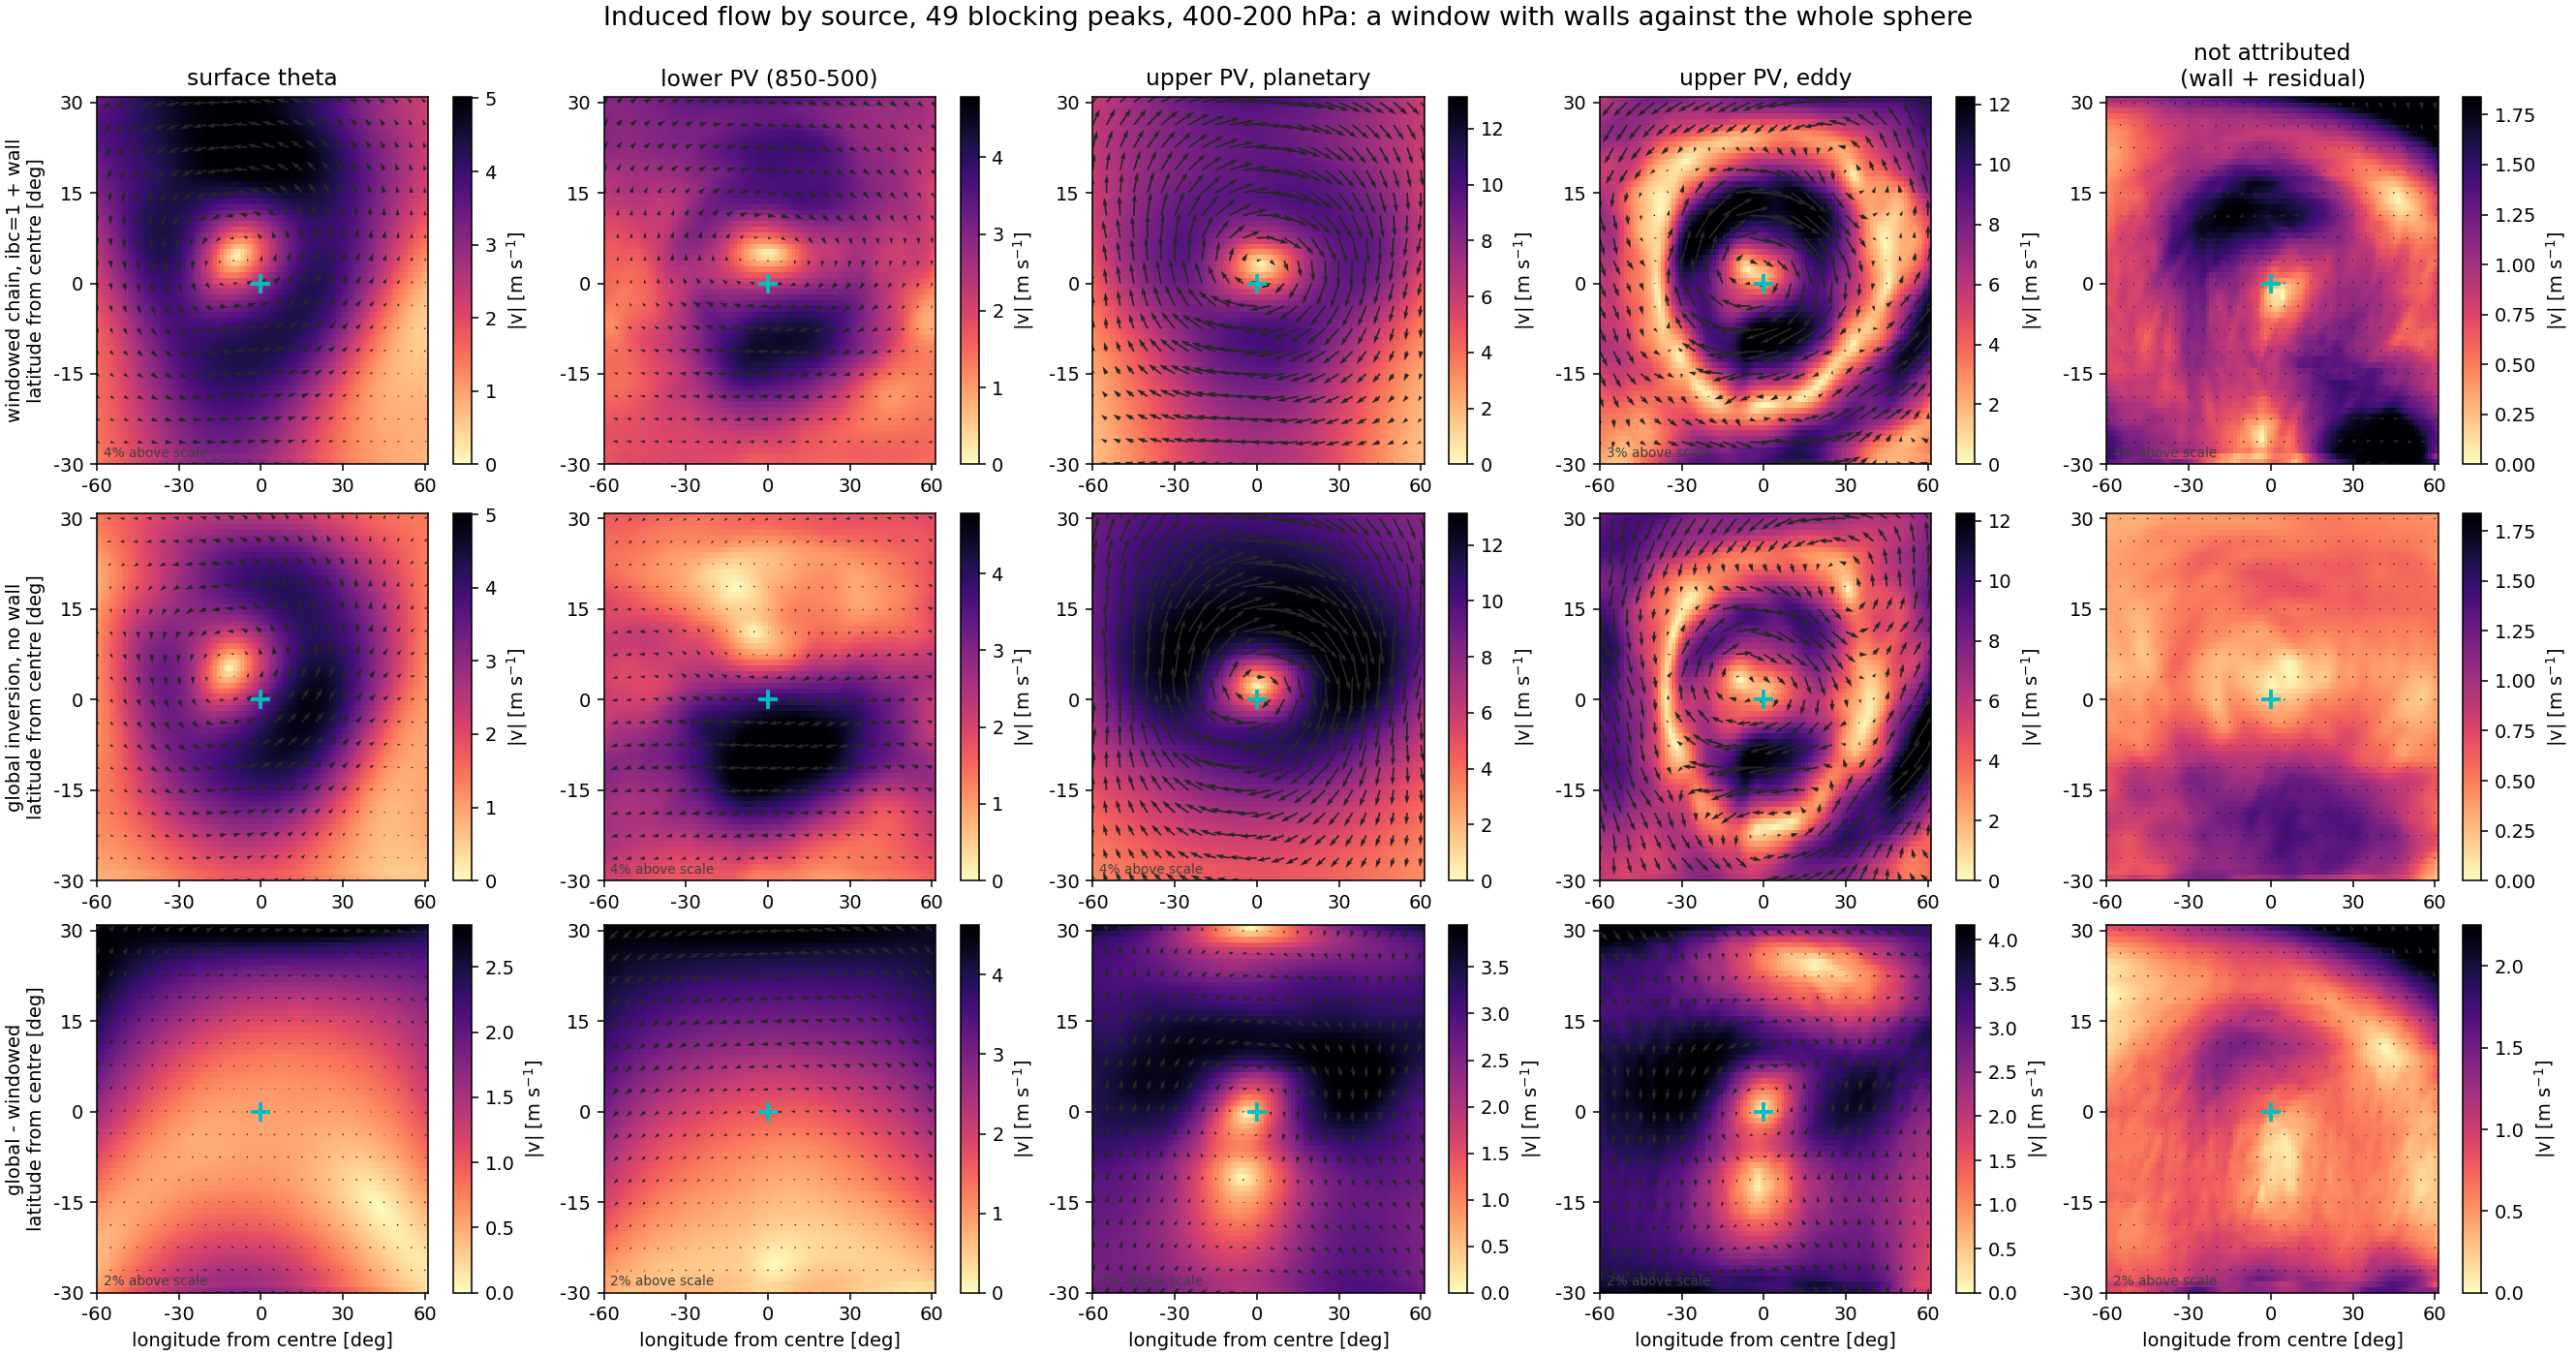
\includegraphics[width=0.9\linewidth]{../examples/03_composite_comparison/fig1_composite_flow.png}
\caption{Fifty blocking peaks, composite of the induced flow at 400--200\,hPa
on the event-centred patch. Columns: the surface, lower, upper-planetary and
upper-eddy pieces, and the part not attributed to any source. Rows: the
windowed chain (\code{ibc=1}, wall piece included in the last column), the
global inversion, and their difference.}
\label{fig:composite}
\end{figure}

\textbf{Fifty events.} Both chains decompose the same balanced perturbation
into the same four sources (Figure~\ref{fig:composite}). On the common patch,
rms in m~s$^{-1}$, the windowed chain attributes 3.45 to the surface, 2.66 to
the lower levels, 7.56 to the planetary and 6.74 to the eddy upper piece, and
leaves 1.09 unattributed, of which 0.79 is its wall piece and 0.99 its
residual, against a reference anomaly of 10.14. The global inversion
attributes 3.03, 2.61, 8.65 and 6.86 and leaves 0.26, 2.6\% of its 10.12
anomaly. Removing the boundary moves the flow from the unattributed part and
the surface into the planetary upper-level piece; the eddy and lower pieces
barely change.

\begin{figure}[htbp]
\centering
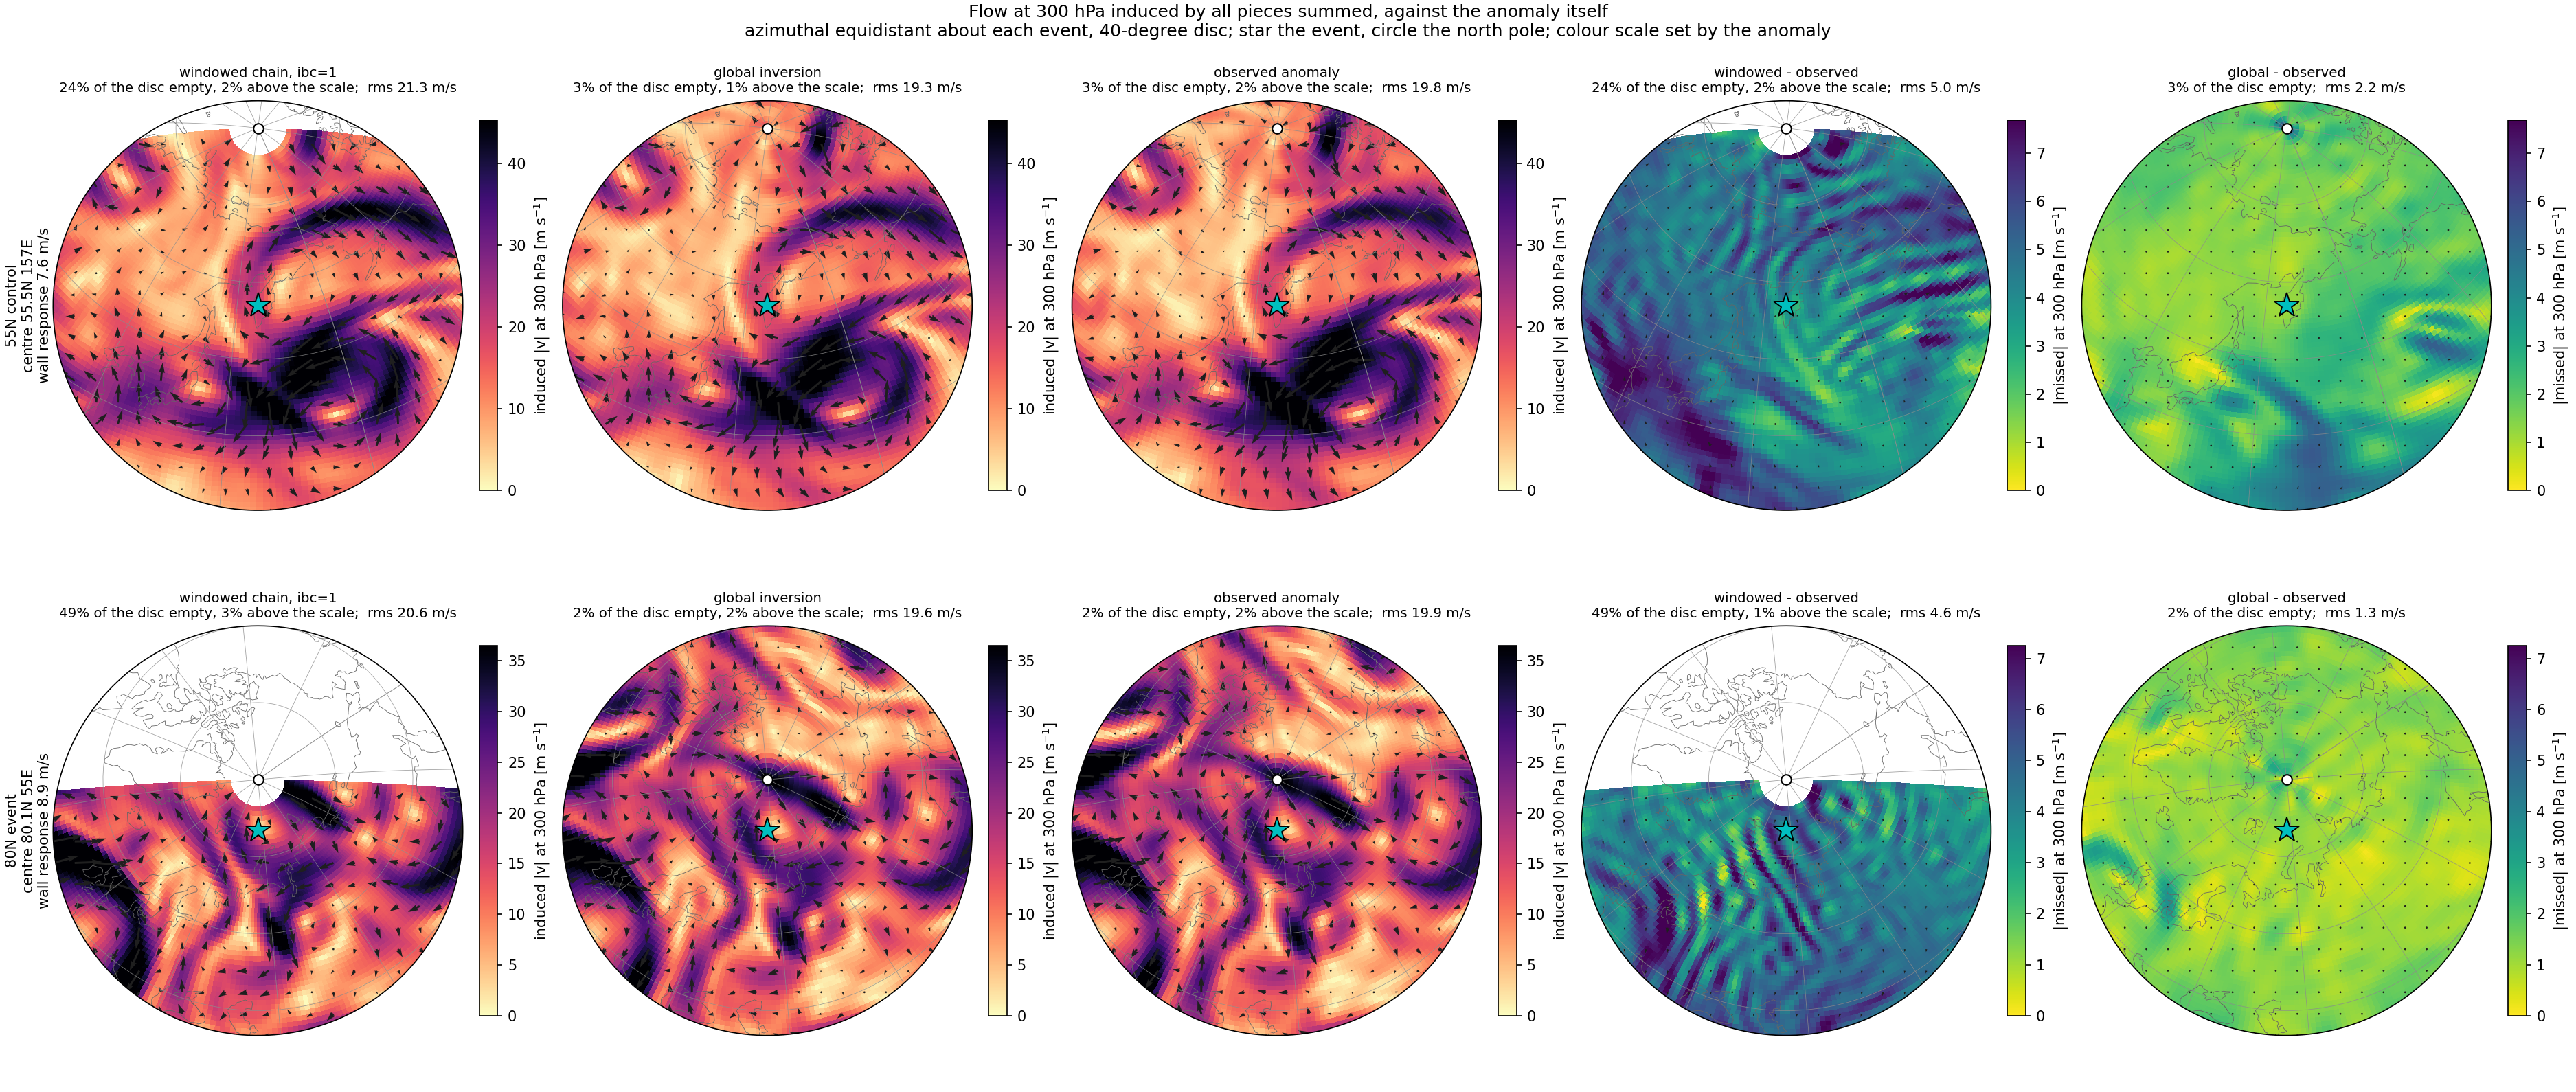
\includegraphics[width=0.95\linewidth]{../examples/02_polar_event/polar_cap.png}
\caption{Two events, at 55\,N and 80\,N: the 300\,hPa flow induced by all
pieces summed, for the windowed chain and the global inversion, beside the
observed anomaly and the two differences from it, on a 40-degree disc about
each centre. Star: the event; white circle: the North Pole.}
\label{fig:polarcap}
\end{figure}

\textbf{Two events near the pole.} For the control at 55~N and the event at
80~N (Figure~\ref{fig:polarcap}) the windowed chain cannot reach 24\% and 49\%
of the disc, and misses the observed anomaly by 5.0 and 4.6~m~s$^{-1}$ rms
where it does reach. The global inversion converges in four Newton steps for
both, leaves 3\% and 2\% of the disc empty, the pole row, and misses by 2.2 and
1.3~m~s$^{-1}$.

% =============================================================================
\section{Running it}
\label{sec:running}

\textbf{Install.} \code{pip install -e .}; NumPy, SciPy (1.12 or newer, for
the \code{rtol} keyword of the Krylov drivers), threadpoolctl, xarray and
netCDF4; matplotlib and cartopy for the figures only.

\textbf{Input contract.} Each state is four arrays of shape
$(n_{\text{lev}},n_{\text{lat}},n_{\text{lon}})$ over the northern hemisphere:
\code{lat} ascending from the equator to 90~N, either on the equator or half a
step from it; \code{lon} ascending from 0; \code{level} descending in pressure,
1000~hPa first; \code{z} a geopotential \emph{height} in metres; \code{t} a
\emph{temperature} in kelvin; \code{u}, \code{v} in m~s$^{-1}$. The
climatology is on the same grid and levels. The geopotential and the
temperature must be hydrostatically consistent (Step~2).

\textbf{One event, from Python.}
{\small
\begin{verbatim}
from pvinv_sph.config import InversionConfig, MirrorConfig
from pvinv_sph.levels import build_levels
from pvinv_sph.passd import invert_pieces
from pvinv_sph.prepare import prepare_state
from pvinv_sph.sht import SHT, gaussian_grid
from pvinv_sph.sphere import SphereOps
from pvinv_sph.winds import rotational_wind_stack

levels = build_levels("NL9")
solver = SphereOps(SHT(gaussian_grid(96, 192), lmax=63))
cfg    = InversionConfig(mirror=MirrorConfig(blend=True))

event = prepare_state(z_ev, t_ev, u_ev, v_ev, lat, lon, levels, solver)
clim  = prepare_state(z_cl, t_cl, u_cl, v_cl, lat, lon, levels, solver)
result = invert_pieces(solver, levels, clim, event, cfg=cfg)

# the rotational wind induced by the 300 hPa potential-vorticity anomaly
u, v = rotational_wind_stack(solver, result.pieces["300"].psi_spec)
\end{verbatim}
}
\code{result.pieces} is keyed by pressure in hPa, \code{"1000"} and
\code{"100"} being the boundary pieces; \code{result.diagnostics} carries the
Newton history, the Krylov count per piece, the posed-equation residuals and
the limiter and clamp reports; \code{result.summed\_psi()} is compared with
\code{all\_sources\_inversion} for the closure of Step~6. For the patch
cropping and the output arrays use \code{invert\_event} from
\code{pvinv\_sph.pipeline}.

\textbf{A catalogue, from the command line.} The command of Step~8, with the
flags
\begin{center}
\small
\begin{tabularx}{\linewidth}{>{\raggedright\arraybackslash}p{4.7cm}>{\raggedright\arraybackslash}p{1.9cm}L}
\toprule
flag & default & meaning \\
\midrule
\code{--pieces} & \code{per\_level} & \code{per\_level} or \code{scale} (Step~5); disjoint key sets, not to be mixed in one directory \\
\code{--pv-source} & \code{operator} & stencils of the potential-vorticity source (Step~2) \\
\code{--deformation-limiter} & \code{adaptive} & \code{adaptive}, \code{observed} or \code{off} (Step~3) \\
\code{--krylov-maxiter} & 800 & operator applications per linear solve \\
\code{--newton-max-steps} & 20 & cap on the nonlinear iteration \\
\code{--blend-south}, \code{--blend-north} & 5.0, 20.0 & edges of the equatorial weight, degrees \\
\code{--f-floor-deg} & 12.0 & latitude scale of the Coriolis floor \\
\code{--rotated-track} & --- & also write the rotated-frame patch \\
\code{--solver-nlat}, \code{--solver-nlon} & 128, 256 & the Gaussian solver grid \\
\code{--lat-half}, \code{--lon-half} & 30.0, 60.0 & output patch half-widths \\
\code{--workers}, \code{--skip-existing} & CPU count, --- & processes; resume a run \\
\bottomrule
\end{tabularx}
\end{center}
A run that hits the Newton cap is reported, not raised: read
\code{meta\_newton\_final\_increment\_m} and the posed-equation residuals
before treating it as a failure. A solution quoted equatorward of about 20~N
lies inside the Coriolis floor and the weight, and is to be checked against a
run with a smaller \code{--f-floor-deg} and a narrower band.

\textbf{Tests and figures.}
{\small
\begin{verbatim}
PYTHONPATH=src python -m pytest tests -q
python examples/01_walkthrough/build.py
jupyter nbconvert --to notebook --execute --inplace \
    --ExecutePreprocessor.timeout=3600 \
    examples/01_walkthrough/01_walkthrough.ipynb
\end{verbatim}
}
The tests check the vertical stencil, the boundary folding, the balance term
against solid-body rotation and under rotation of a vortex to the pole, the
spectral round trip, the midpoint identity with the weight on, the limiter and
its Jacobian, the pieces' thermal-wind boundary levels, and the closure of the
pieces against the all-sources solve. The notebook produces every figure of
Section~\ref{sec:steps}.

% =============================================================================
\begin{thebibliography}{9}

\bibitem{charney1955}
Charney, J., 1955:
The Use of the Primitive Equations of Motion in Numerical Prediction.
\emph{Tellus}, \textbf{VII}(1), 22--26.

\bibitem{de1991}
Davis, C. A., and K. A. Emanuel, 1991:
Potential Vorticity Diagnostics of Cyclogenesis.
\emph{Monthly Weather Review}, \textbf{119}(8), 1929--1953.

\bibitem{davis1992}
Davis, C. A., 1992:
Piecewise Potential Vorticity Inversion.
\emph{Journal of the Atmospheric Sciences}, \textbf{49}(16), 1397--1411.

\end{thebibliography}

\end{document}
